
\chapter{Grundlagen}


\section{ABB}

ABB ist ein global f\"{u}hrender Hersteller und Serviceanbieter in der Energie- und Automatisierungstechnik mit Hauptsitz in Z\"{u}rich.
Der internationale Konzern entstand 1988 aus der Fusion des schwedischen Unternehmens \ac{ASEA} und der schweizerischen Firma \ac{BBC}. ABB besch\"{a}ftigt zurzeit \"{u}ber 132.000 Mitarbeiter in 100 L\"{a}ndern. Im Jahr 2016 wurde ein weltweiter Umsatz von 33,8 Mrd. USD und ein Nettogewinn von 2,1 Mrd erwirtschaftet.\footnote{Vgl. ABB Gesch\"{a}ftsbericht 2016} 
\linebreak



\begin{figure}[ht]
	\centering
	\makebox[\textwidth][c]{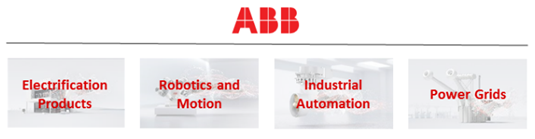
\includegraphics[width=1\textwidth]{img/ABB-Div.png}}%
	
	\caption{Divisionen von ABB}
	\label{fig1}
	
\end{figure}

Das Produktportfolio von ABB gliedert sich in vier Divisionen auf: Division Electrification, Robotics and Motion, Industrial Automation und Power Grids. Diese Aufteilung ist auch in Abbildung \ref{fig1} zu sehen.


\section{SAP}

Die folgende Arbeit findet fast ausschließlich in der \ac{ERP} Software SAP statt. SAP wird in fast 50\% aller Firmen mit einer Mitarbeiterzahl von \"{u}ber 500 genutzt.
SAP kann in drei Schichten unterteilt werden: Die Pr\"{a}sentations-, Anwendungs- und Datenbankschicht \\
\begin{figure}[ht]
	\centering
	\makebox[\textwidth][c]{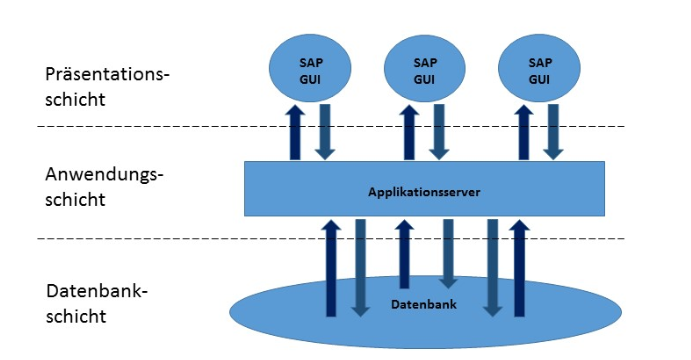
\includegraphics[width=1.2\textwidth]{img/SAP-Schicht.png}}%
	
	
	\caption{Aufbau des ERP Systems SAP}
	\label{fig2}
	
\end{figure}
\\
Die Datenbankschicht besteht aus einer relationalen SQL Datenbank, welche alle Daten des SAP Systems beinhaltet. Die Verarbeitung dieser Daten findet in der Anwendungsschicht statt. Mit Hilfe der von SAP eigens entwickelten Programmiersprache \ac{ABAP} werden hier Daten zusammen mit Anweisungen aus der Pr\"{a}sentationsschicht verarbeitet. Die Pr\"{a}sentationsschicht stellt das SAP-System grafisch \"{u}ber ein \ac{GUI} dar, durch welches der Anwender komfortabel auf das SAP System zugreifen kann. \medskip 

Das SAP-System ist in unterschiedliche Module unterteilt. Jedes dieser Module deckt verschiedene Prozesse und Funktionen ab. Die wichtigsten Module sind unter den \"{U}berschriften Logistikmodule und kaufm\"{a}nnische Module zusammengefasst. Zus\"{a}tzlich existiert außerhalb dieser Gruppierung das \ac{HR} Modul. 
Die Gruppe Logistikmodule beinhaltet das \ac{SD}, \ac{MM} , \ac{PP}, \ac{PM}, \ac{CS}, \ac{GTS} und das \ac{QM} Modul. Da nicht alle Unternehmen die gleichen Prozesse nutzen, werden jeweils nur die notwendigen Module dieser Auswahl eingesetzt. 
Alle kaufm\"{a}nnischen Prozesse werden dann mit Hilfe der kaufm\"{a}nnischen Module dargestellt. Diese beinhalten das \ac{FI}, \ac{CO} und \ac{AA} Modul.

Die folgende Arbeit bezieht sich auf dein Dokument welches im \ac{GTS} Modul erstellt wird.  




\section{Smartforms}
Die, bei ABB am meist genutzte, Technologie zur Dokumenterstellung im SAP ist die der Smartforms. Mit Hilfe des Layout-Painters wird hierbei die Oberfläche des Dokumentes gestaltet und konfiguriert. 

\section{Adobe PDF}

\section{Dokumente im SAP}